% Copyright 2007 by Till Tantau
%
% This file may be distributed and/or modified
%
% 1. under the LaTeX Project Public License and/or
% 2. under the GNU Public License.
%
% See the file doc/licenses/LICENSE for more details.



\documentclass{beamer}

%
% DO NOT USE THIS FILE AS A TEMPLATE FOR YOUR OWN TALKS�!!
%
% Use a file in the directory solutions instead.
% They are much better suited.
%


% Setup appearance:

\usetheme{Darmstadt}
\usefonttheme[onlylarge]{structurebold}
\setbeamerfont*{frametitle}{size=\normalsize,series=\bfseries}
\setbeamertemplate{navigation symbols}{}


% Standard packages

\usepackage[english]{babel}
\usepackage[latin1]{inputenc}
\usepackage{times}
\usepackage[T1]{fontenc}

% Setup TikZ

\usepackage{tikz}
\usetikzlibrary{arrows}
\tikzstyle{block}=[draw opacity=0.7,line width=1.4cm]


% Author, Title, etc.

\title[Distributed $3$D-Print Driver] 
{%
 Distributed \textbf{$3$}D-Print Driver
 %
}

\author[Guide]{
	\textbf{Presenter}: Suman~Bidarahalli \\	
	\textbf{Supervisor}: Dr.Alan~Brunton 
}
\institute[TU Darmstadt]
{
  Technische Universit�t Darmstadt, Germany
}

\date[ Master Thesis Presentation 2016]
{Master Thesis Presentation, August 2016}



% The main document

\begin{document}

\begin{frame}
  \titlepage
\end{frame}

\begin{frame}{Outline}
  \tableofcontents
\end{frame}


\section{Introduction}

\subsection{State of the art $3$D Print Driver}

\begin{frame}{Motivation}

\begin{columns}
    \begin{column}{0.25\textwidth}
    \centering
    \begin{figure}[!ht]
			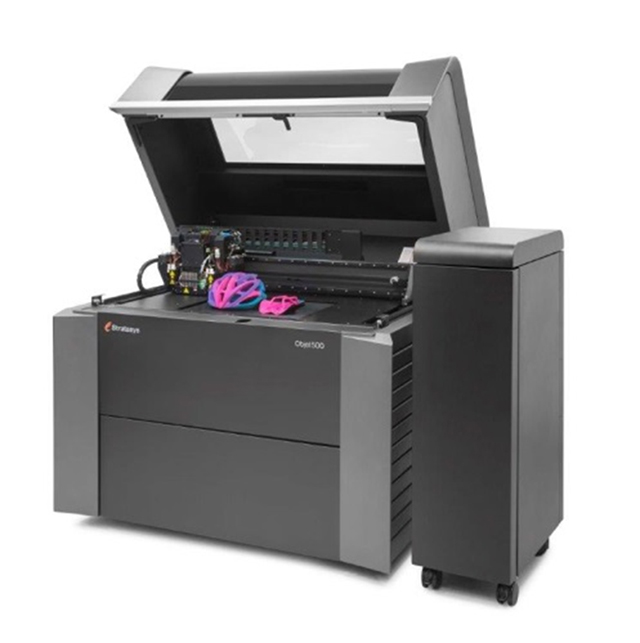
\includegraphics[width=0.90\textwidth]{PrinterI}
			\caption{State of the art $3$D Printers}
			\label{Fig:State of the art $3$D Printers}
		\end{figure}
    \end{column}
    \begin{column}{0.75\textwidth}
    \centering
    \begin{itemize}
			\item Today's $3$D Printers allow for multi-material high resolution prints(today up to 7 materials can be combined in a single printout)
			\item Multiple objects in varying size can be printed at a go
			\item Voxel-level material assignment enables to reproduce an object's color, shape, texture, gloss,and translucency with high-fidelity
			\item Larger print objects are composed of huge number of voxels( can easily cross \begin{math}10^{12}\end{math} voxels per object)
		\end{itemize} 
    \end{column}
  \end{columns}
\end{frame}

\subsection{Problem Statement}

\begin{frame}[t]{Why do we need a distributed $3$D Print Driver?}
\begin{columns}
    \begin{column}{0.45\textwidth}
    \centering
    \begin{figure}[!ht]
			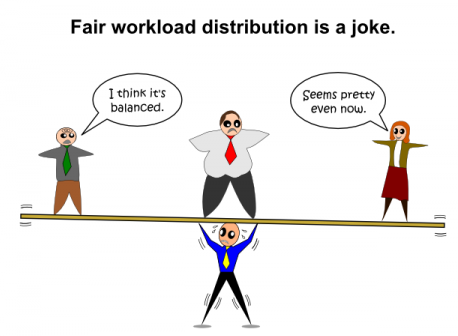
\includegraphics[width=0.90\textwidth]{SillyImage}
			\label{Fig:MythI}
		\end{figure}
    \end{column}
    \begin{column}{0.55\textwidth}
    \centering
    \begin{itemize}
    \item Bigger prints require large amount of computational effort 
    \item Single workstation is limited in terms of resources  
		\item Cuttlefish processes the input in a serial fashion leading to increased computation time for higher number of models
    \item Distributed computing is one way of achieving better performance for large computations 
		\end{itemize} 
    \end{column}
  \end{columns}
\end{frame}

\section{Solution}

\subsection{Where is the distribution of the workload done?}
\begin{frame} {Infrastructure for distribution}
\begin{columns}
  \begin{column}{0.50\textwidth}
  \centering
	\begin{figure}[!ht]
			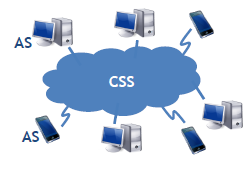
\includegraphics[width=0.90\textwidth]{DistributeIII}
			\caption{Distributed System}
			\label{Fig:DistributeIII}
		\end{figure}
	\end{column}
	\begin{column}{0.50\textwidth}
  \begin{itemize}
		\item The distribution of the workload is done amongst the nodes of the cluster
		\item A \textbf{\textit{distributed system}} is a cluster of AS where each AS is connected to other by a network and primarily communicate via message passing
	\end{itemize} 
	\end{column}
\end{columns}
\end{frame}

\begin{frame}{Currently used Distributed System}
\begin{columns}
  \begin{column}{0.50\textwidth}
  \centering
    \begin{figure}[!ht]
			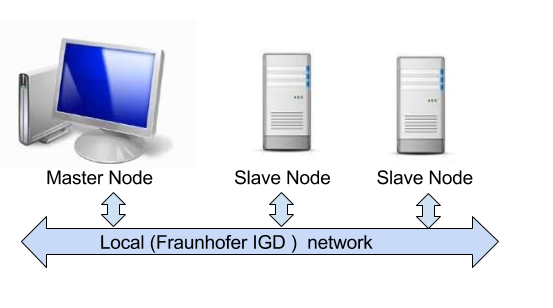
\includegraphics[width=0.90\textwidth]{ArchitectureI}
			\caption{Distributed Systems Architecture}
			\label{Fig:ArchitectureI}
		\end{figure}
	\end{column}
	\begin{column}{0.50\textwidth}
	\begin{itemize}
	\item The distributed system used to implement the solution consists of $3$ nodes - a master node and two slave nodes
	\item The nodes are connected via local(Fraunhofer) network
	\item All the nodes also have access to a shared network file system
	\end{itemize}	
	\end{column}
\end{columns}
\end{frame}

\begin{frame}{Task Submission \& Distribution}
\begin{columns}
  \begin{column}{0.50\textwidth}
  \centering
    \begin{figure}[!ht]
			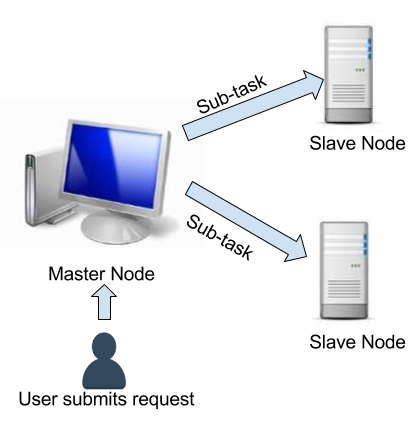
\includegraphics[width=0.90\textwidth]{ArchitectureII}
			\caption{Task Submission}
			\label{Fig:ArchitectureII}
		\end{figure}
	\end{column}
	\begin{column}{0.50\textwidth}
	\begin{itemize}
	\item The submission of the task is done at the master node
	\item The master node is responsible for the division of the submitted task into sub-tasks
	\end{itemize}	
	\end{column}
\end{columns}
\end{frame}

\begin{frame}{Sub-Task Computation \& Partial Results Reporting}
\begin{columns}
  \begin{column}{0.50\textwidth}
  \centering
    \begin{figure}[!ht]
			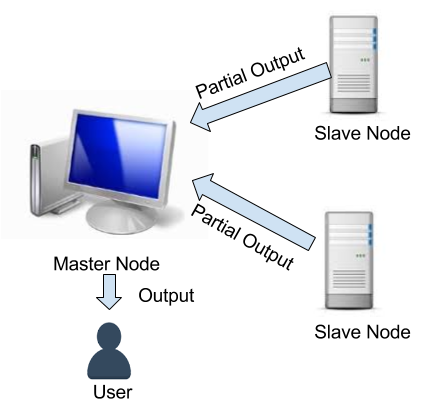
\includegraphics[width=0.90\textwidth]{ArchitectureIII}
			\caption{Sub-Task Computation}
			\label{Fig:ArchitectureIII}
		\end{figure}
	\end{column}
	\begin{column}{0.50\textwidth}
	\begin{itemize}
	\item The slave nodes perform the computation locally
	\item The output of the computation performed by the slaves is then reported back to the master node
	\item The master node may perform final computation using the received partial output from the slaves and provide the user with the final output
	\end{itemize}	
	\end{column}
\end{columns}
\end{frame}

\subsection{How is the distribution done?}
\begin{frame}{Different possibilities of distribution}
\begin{columns}
   \begin{column}{0.50\textwidth}
    \centering
    \begin{figure}[!ht]
			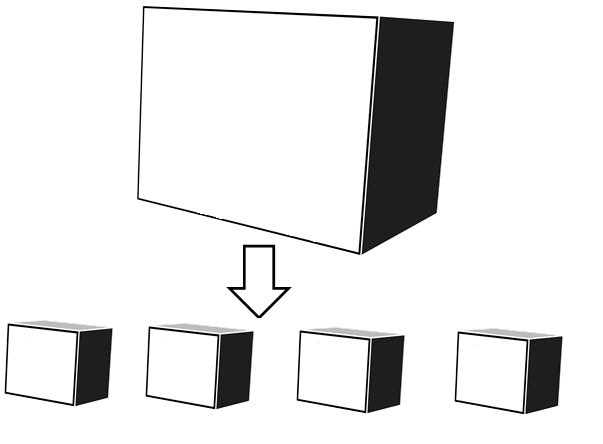
\includegraphics[width=0.30\textwidth]{DistributeI}
			\caption{Distribute Single Large Print Object}
			\label{Fig:DistributeI}
		\end{figure}
		\begin{figure}[!ht]
			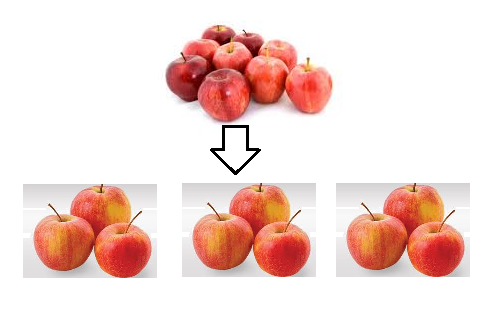
\includegraphics[width=0.70\textwidth]{DistributeII}
			\caption{Distribute Multiple Print Objects}
			\label{Fig:DistributeII}
		\end{figure}
   \end{column}
	\begin{column}{0.50\textwidth}
    \centering
    \begin{itemize}
		\item Distribution of one large print object amongst the workstations 
		\item Distribution of multiple print objects amongst the workstations
		\end{itemize} 
    \end{column}
  \end{columns}
  \end{frame}

\begin{frame}{Chosen distribution}
    \begin{itemize}
		\item Multiple print objects will be distributed amongst the workstations i.e. each workstation performs computation on one or more whole inputs
		\item The distribution of the workload and the collection of partial results is done through MPI(Message Passing Interface)
		\end{itemize}
\end{frame}

\subsection{Who distributes the workload?}
\begin{frame}{Current Component Architecture}
\begin{block}{Streaming Architecture}
	\begin{figure}[!ht]
		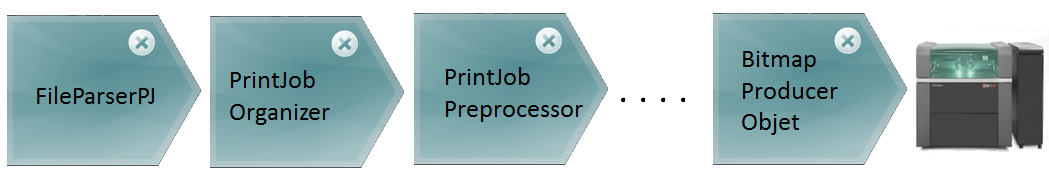
\includegraphics[width=0.9\textwidth]{StreamingArchitectureI}
		\caption{Cuttlefish- Streaming Architecture}
		\label{Fig:StreamingArchitectureI}
	\end{figure}
\end{block}
	\begin{itemize}
		\item Cuttlefish Streaming architecture enables to perform the computation serially in a chunk-wise manner for each print object 
		\item Goal: To retain the architecture and provide distinguished components to handle the distribution of sub-tasks and collection of the partial results
	\end{itemize} 
\end{frame}

\begin{frame}{Modified Component Architecture- I}
\begin{block}{Streaming Architecture- Master Printing Software }
	\begin{figure}[!ht]
		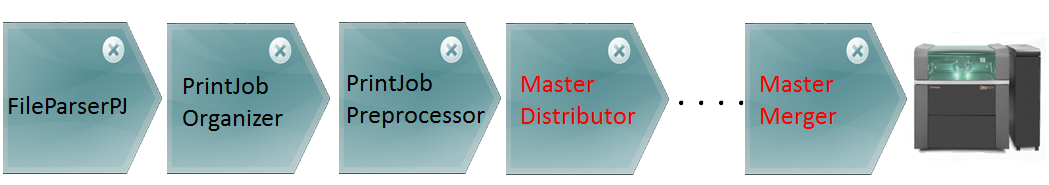
\includegraphics[width=0.9\textwidth]{StreamingArchitectureII}
		\caption{Cuttlefish Streaming Architecture- Master}
		\label{Fig:StreamingArchitectureII}
	\end{figure}
\end{block}
	\begin{itemize}
		\item The components of the printing software are decided depending on the rank of the node 
		\item Master node(rank=0 in the cluster) runs the \textit{\textbf{Master Printing Software}} with the components as shown in the above figure. 
		\item Additional components introduced-\textbf{ \textit{Master Distributor}} \& \textbf{\textit{Master Merger}}
	\end{itemize} 
\end{frame}

\begin{frame}{Master Distributor}
	\begin{itemize}
		\item Computes the cost function used to perform a \textit{fair} distribution amongst the slaves
		\item Distribution of the sub-task is done through writing the main\_conf.json file per slave node  
	\end{itemize} 
\end{frame}

\begin{frame}{Cost function}
\begin{itemize}
	\item For each object \textit{i}, compute the minimum bounding box(\begin{math}b_{min}^i\end{math}) and maximum bounding box(\begin{math}b_{max}^i\end{math})
	\item Using \begin{math}b_{min}^i\end{math} and \begin{math}b_{max}^i\end{math}, calculate the width(w), height(h),and length(l)
	\begin{itemize}
		\item w=\begin{math}(b_{max}^i).y-(b_{min}^i).y\end{math} 
		\item h=\begin{math}(b_{max}^i).z-(b_{min}^i).z\end{math}
		\item l=\begin{math}(b_{max}^i).x-(b_{min}^i).x\end{math}
	\end{itemize}
	\item Volume of the object \begin{math}V^i= w*h*l\end{math}
	\item Total Volume(k objects)=\begin{math}\sum\limits_{i=1}^{k}{V^i}\end{math}
	\item Threshold (for cluster size n-1)=\begin{math}(\sum\limits_{i=1}^{k}{V^i})/(n-1)\end{math}
	\item Each slave node is allocated objects until the sum of the allocated object volume does not exceed the calculated threshold
\end{itemize}
\end{frame}		

\begin{frame}{Master Merger}
	\begin{itemize}
		\item Collects the partial output from the slaves
		\item De-serializes the partial output and merges the partial slices to construct full slices  
	\end{itemize} 
\end{frame}

\begin{frame}{Modified Component Architecture- II}
\begin{block}{Streaming Architecture- Slave Printing Software }
	\begin{figure}[!ht]
		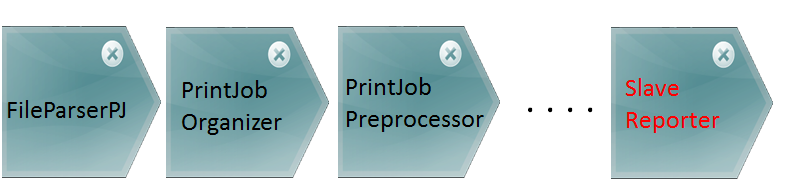
\includegraphics[width=0.9\textwidth]{StreamingArchitectureIII}
		\caption{Cuttlefish Streaming Architecture- Slave}
		\label{Fig:StreamingArchitectureII}
	\end{figure}
\end{block}
	\begin{itemize}
		\item Nodes with rank$>$$0$ are slave nodes which run the \textit{\textbf{Slave Printing Software}}
		\item Additional component introduced-\textbf{ \textit{Slave Reporter}}
	\end{itemize} 
\end{frame}

\begin{frame}{Slave Reporter}
	\begin{itemize}
		\item Each Slave node after performing the computation has chunk-wise partial output in form of slices 
		\item Slave reporter component serializes the slices and sends the data to the master
		\item The serialized data is currently written to the shared network file system and the slave sends the path to the master
	\end{itemize} 
\end{frame}

\section{Current Task}
\subsection{Merging of the sub-slices}
\begin{frame}{Unequal number of slices introduces some challenges}
Cases that need to be addressed while merging unequal number of slices  
	\begin{itemize}
		\item One/ Many slaves report last chunk with less number of slices
		\item Some slave nodes finish computation earlier as the object size is smaller leading to only remaining slaves reporting the pending slices. So the master needs to be aware of this information so as to merge the slices correctly
	\end{itemize} 
\end{frame}

\section{Pending Work}
\subsection{Fair Distribution}
\begin{frame}{Implementation of multiple cost functions}
\begin{itemize}
\item Distribution of the workload among the slaves needs to be fair 
\item Various parameters other than the volume of the object can be used to determine the division of workload  
\item Design and implement additional cost functions 
\end{itemize} 
\end{frame}

\subsection{Sub-task distribution}
\begin{frame}{Serialize \& De-serialize Print Jobs }
	\begin{itemize}
		\item Sub-Tasks are currently distributed through writing the main\_conf.json file for each slave
		\item This leads to redundant execution of FileParserPJ, PrintJobOrganizer and PrintJobPreprocessor at the slave
		\item Serialized PrintJob can be instead sent to the slave nodes which would then be de-serialized and proceed with the computation 
	\end{itemize} 
\end{frame}

\subsection{Partial Output collection}
\begin{frame}{Serialize \& De-serialize Slices }
	\begin{itemize}
		\item Partial Output from the slave is currently reported to the master through writing serialized slices to a file 
		\item Serialization of the slices to bytes which can be directly sent to the master through MPI\_SEND call
		\item Similarly at the Master, buffering of the received bytes and de-serialization to partial slices needs to implemented
	\end{itemize} 
\end{frame}

\subsection{Evaluation}
\begin{frame}{Performance Gain and Management Overhead}
	\begin{itemize}
		\item Evaluation of the various designs by comparing the performance gains
		\item Evaluation of the design by comparing the overhead (in terms of extra operations performed (reading/writing to file) or synchronization)
		\item Checking if the generated full slices at the master are correct and try a sample print
	\end{itemize} 
\end{frame}

\section*{Summary}
\begin{frame}
  \frametitle<presentation>{Summary}
	\begin{itemize}
		\item Large computations can be performed on a cluster of nodes by dividing the task to sub-tasks 
		\item Primary goal is to achieve higher resource utilization along with better performance by reducing the computation time
		\item Develop an elegant solution to achieve the goal as well as maintaining the cuttlefish streaming architecture 
		\item To get an overall understanding of the benefits as well as challenges of distributed computing  
	\end{itemize} 
\end{frame}

\appendix
\section*{Appendix} 
\end{document}


